\chapter{Time Series Regression}
\section{Autocorrelation and Empirical Autocorrelation}
Usually through either detrending or differencing, we arrive
at a series $ \set{X_t}_{t\in\mathbf{Z}} $ that we may consider as stationary.

Given such a series, we wish to estimate a function $ g $, so that
\[ X_t=g(W_t,W_{t-1},\ldots) \]
$ \set{W_t}_{t\in\mathbf{Z}} $ is a ``innovation'' sequence (strong white noise)
which could admit serial dependence, etc.

In a first pass, it's reasonable to assume that $ g $ is a linear function.

\begin{Definition}{Linear process}{}
    A time series $ \set{X_t}_{t\in\mathbf{Z}} $ is said to be a
    \textbf{linear process} if there exists a strong
    white noise $ \set{W_t}_{t\in\mathbf{Z}} $ and coefficient
    $ \set{\psi_\ell}_{\ell\in\mathbf{Z}} $
    where $ \psi_\ell\in\mathbf{R} $, so that
    \[ \sum_{\ell=-\infty}^{\infty} \abs{\psi_\ell}<\infty \]
    and
    \[ X_t=\sum_{\ell=-\infty}^{\infty} \psi_\ell W_{t-\ell} \]
    Note that the sum defining $ X_t $ is well-defined
    as a limit in $ L^2 $. Also, we
    must require that $ \Var{W_{t-\ell}}<\infty $.
\end{Definition}
\begin{Definition}{Causal linear process}{}
    We say $ \set{X_t}_{t\in\mathbf{Z}} $ is a \textbf{causal
        linear process} if
    \[ X_t=\sum_{\ell=0}^{\infty} \psi_\ell W_{t-\ell} \]
    Note that $ X_t $ only depends on $ W $'s in the ``past.''
\end{Definition}
\begin{Example}{}{}
    $ X_t=W_t $ is a linear process, so all
    $ \psi $'s are $ 0 $, except for $ \psi_0=1 $
    which is a strong white noise sequence.
\end{Example}
\begin{Remark}{}{}
    Linear processes are \textbf{strictly stationary} since they
    can be written as Bernoulli-shifts.
\end{Remark}
\begin{Example}{}{}
    $ X_t=W_t+\theta W_{t-1} $ where $ \set{W_t}_{t\in\mathbf{Z}} $ is a strong white noise
    with finite variance, and $ X_t $ is a linear process.
    \[ \gamma_X=\begin{cases}
            (1+\theta^2)\sigma_W^2 & h=0     \text{always non-zero} \\
            \theta\sigma_W^2       & h=1                            \\
            0                      & h\ge 2
        \end{cases} \]
    $ \gamma_X(h) $ non-zero for $ h\ge 1 $
    only where ``lagged'' terms in the linear process
    are non-zero. Suggests a way of sleuthing out what
    \[ g(W_t,W_{t-1},\ldots)=\sum_{\ell=0}^{\infty} \psi_\ell W_{t-\ell} \]
    must look like.
\end{Example}
\begin{Definition}{Autocorrelation function}{}
    Suppose $ \set{X_t}_{t\in\mathbf{Z}} $ is weakly stationary. The
    \textbf{autocorrelation function} (ACF) of $ \set{X_t}_{t\in\mathbf{Z}} $
    is
    \[ \rho_X(h)=\frac{\gamma(h)}{\gamma(0)} \quad (h\ge 0) \]
    Note since $ \gamma(0)=\Var{X_t}=\Var{X_0} $ (since the process is stationary),
    \[ \abs{\gamma(h)}=\abs{\Cov{X_t,X_{t+h}}}\Uunderbracket{\le}_{\text{CS}}
        \sqrt{\Uunderbracket{\Var{X_t}\Var{X_{t+h}}}_{\text{Same \# by stationarity}}}=\Var{X_0} \]
    Hence, $ \abs{\rho(h)}\le 1\implies -1\le \rho(h)\le 1 $.
\end{Definition}
\underline{Estimating $ \gamma(h) $ and $ \rho(h) $}:
\[ \gamma(h)=\Cov{X_t,X_{t+h}}=\E{(X_t-\mu)(X_{t+h}-\mu)} \]
where $ \mu=\E{X_t} $. Hence, a sensible estimator is
\[ \hat{\mu}=\frac{1}{T} \sum_{t=1}^{T} X_t=\bar{X} \]
which is the \textbf{sample mean} (\textbf{time series average}).
\[ \hat{\gamma}(h)=\frac{1}{T} \sum_{t=1}^{T-h}(X_t-\bar{X})(X_{t+h}-\bar{X})
    \approx \frac{1}{T-h} \sum_{t=1}^{T-h}(X_t-\bar{X})(X_{t+h}-\bar{X})  \]
where $ (X_t-\bar{X})(X_{t+h}-\bar{X}) $ is the averaging over
centred terms $ h $-time steps apart.
\[ \hat{\rho}(h)=\frac{\hat{\gamma}(h)}{\hat{\gamma}(0)}  \]
\begin{Example}{}{}
    $ X_t=W_t $ where $ \set{W_t}_{t\in\mathbf{Z}} $ is a strong white noise
    with $ \Var{W_t}=\sigma_W^2<\infty $.
    \[ \gamma_X(h)=\begin{cases}
            \sigma_W^2 & h=0    \\
            0          & h\ge 1
        \end{cases} \]
    Therefore,
    \[ \rho_X(h)=\begin{cases}
            1 & h=0    \\
            0 & h\ge 1
        \end{cases} \]
    Note that it's always the case that
    \[ \rho(0)=\frac{\gamma(0)}{\gamma(0)}=1  \]
\end{Example}
\begin{figure}[!ht]
    \centering
    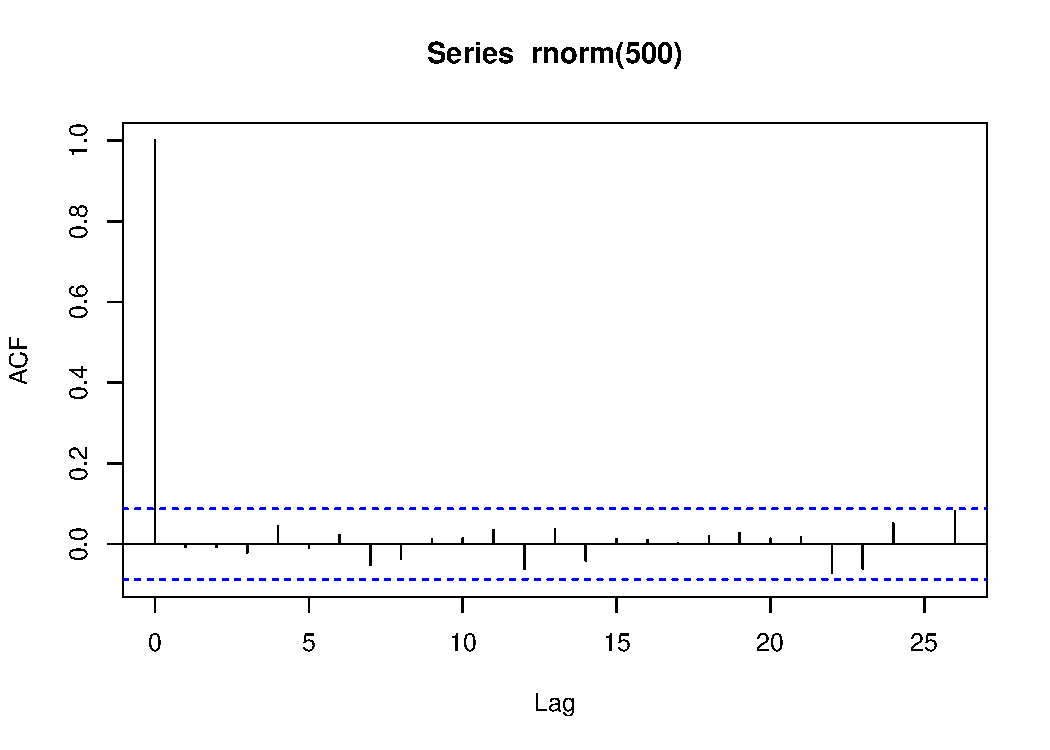
\includegraphics[width=0.75\textwidth]{acfwn130.pdf}
    \caption{Quarterly Johnson and Johnson Earnings}\label{fig:acfwn130}
\end{figure}
\begin{minted}{R}
# Figure 1.8
acf(rnorm(500))
\end{minted}
In Figure~\ref{fig:acfwn130}:
{\color{blue}Let's then have a look at what the empirical autocorrelation
function looks like when we apply it to a strong white noise sample.
In this case, we are considering a strong Gaussian white noise
with variance 1. This is what the sample ACF looks like.
What we're plotting here is on the $ x $-axis we have the lags $ h $,
and on the $ y $-axis we have the magnitudes of the autocorrelation $ \hat{\rho}(h) $.
What we're seeing here
is $ \hat{\rho}(0)=1 $ (by definition). However, for lags other than zero,
for the other autocorrelations plotted, we can see that they are
relatively small compared to $ \hat{\rho}(0)=1 $,
which is the point of the blue lines (explained
in the next lecture). The basic interpretation of blue lines is that
if an autocorrelation would go inside the blue lines then you could imagine
that it would be consistent with the series being a strong white noise,
which is what we observe here. There's small violations that can occur by
sheer chance.}
